\begin{frame}{Is the Adjoint Flow Solved Correctly?}
Not many quantitative solutions of the adjoint field are available.
From \footfullcite{Sorgiovanni2016} 2 adjoint flows are reported.    
\end{frame}


\begin{frame}{Cylinder Reynolds 50}
    \begin{figure}[h]
        \centering          
        \begin{subfigure}[h]{0.45\textwidth}
                 \centering
            \includegraphics[width=\textwidth]{PaperRef/Cylinder_Uadjoint.png}
       \end{subfigure}
       \hfill	
       \begin{subfigure}[h]{0.45\textwidth}
                \centering
           \includegraphics[width=\textwidth]{MyRes/Cylinder_Uadjoint.png}
        \end{subfigure}
        \caption{Adjoint Velocity}
        \end{figure} 
    \end{frame}
    
    \begin{frame}{Cylinder Reynolds 50}
    \begin{figure}[h]
        \centering          
        \begin{subfigure}[h]{0.45\textwidth}
                 \centering
            \includegraphics[width=\textwidth]{PaperRef/Cylinder_Padjoint.png}
       \end{subfigure}
       \hfill	
       \begin{subfigure}[h]{0.45\textwidth}
                \centering
           \includegraphics[width=\textwidth]{MyRes/Cylinder_Padjoint.png}
        \end{subfigure}
        \caption{Adjoint Pressure}
        \end{figure} 
    \end{frame}

\begin{frame}{NACA0012 $AoA=\ang{2.5}$, $Re=1000$}
Drag minimization.
Boundary conditions:
\begin{itemize}
    \item $\Gamma_{airfoil}: \Psi_u = [-1.0, 0.0]$
    \item $\Gamma_{inlet}:\Psi_p = 0.0$
    \item $\Gamma_{outlet}: \Psi_u = [0.0, 0.0]$
    \item $\Gamma_{limits}: \Psi_u = [0.0, 0.0]$

\end{itemize}
        
\end{frame}

\begin{frame}{NACA0012 $AoA=\ang{2.5}$, $Re=1000$}
\begin{figure}[h]
    \centering          
    \begin{subfigure}[h]{0.45\textwidth}
             \centering
        \includegraphics[width=\textwidth]{PaperRef/NACA0012_Uprimal.png}
   \end{subfigure}
   \hfill	
   \begin{subfigure}[h]{0.45\textwidth}
            \centering
       \includegraphics[width=\textwidth]{MyRes/NACA0012_Uprimal.png}
    \end{subfigure}
    \caption{Primal Velocity}
    \end{figure} 
\end{frame}

\begin{frame}
\begin{figure}[h]
    \centering          
    \begin{subfigure}[h]{0.45\textwidth}
             \centering
        \includegraphics[width=\textwidth]{PaperRef/NACA0012_Pprimal.png}
   \end{subfigure}
   \hfill	
   \begin{subfigure}[h]{0.45\textwidth}
            \centering
       \includegraphics[width=\textwidth]{MyRes/NACA0012_Pprimal.png}
    \end{subfigure}
    \caption{Primal Pressure}
    \end{figure} 
\end{frame}

\begin{frame}
\begin{figure}[h]
    \centering          
    \begin{subfigure}[h]{0.45\textwidth}
             \centering
        \includegraphics[width=\textwidth]{PaperRef/NACA0012_Uadjoint.png}
   \end{subfigure}
   \hfill	
   \begin{subfigure}[h]{0.45\textwidth}
            \centering
       \includegraphics[width=\textwidth]{MyRes/NACA0012_Uadjoint.png}
    \end{subfigure}
    \caption{Adjoint Velocity}
    \end{figure} 
\end{frame}

\begin{frame}
\begin{figure}[h]
    \centering          
    \begin{subfigure}[h]{0.45\textwidth}
             \centering
        \includegraphics[width=\textwidth]{PaperRef/NACA0012_Padjoint.png}
   \end{subfigure}
   \hfill	
   \begin{subfigure}[h]{0.45\textwidth}
            \centering
       \includegraphics[width=\textwidth]{MyRes/NACA0012_Padjoint.png}
    \end{subfigure}
    \caption{Adjoint Pressure}
    \end{figure} 
\end{frame}


\begin{frame}{Finite Difference Tests}
Computing the gradients for a STEADY case. NACA0012, $AoA=\ang{0.0}$, Re=100. 
In FD, each $\beta_i$ is perturbed by $\epsilon$ and the flow is solved. 
$$ \dfrac{\partial C_D }{\partial \beta _ i} = \dfrac{C_D'-C_D}{\epsilon}$$

Gradients computed with FD and Adjoind should be the same, but they are not. The perturbation $\epsilon$ is the same for FD and adjoint.
\begin{figure}[h]
    \centering          
        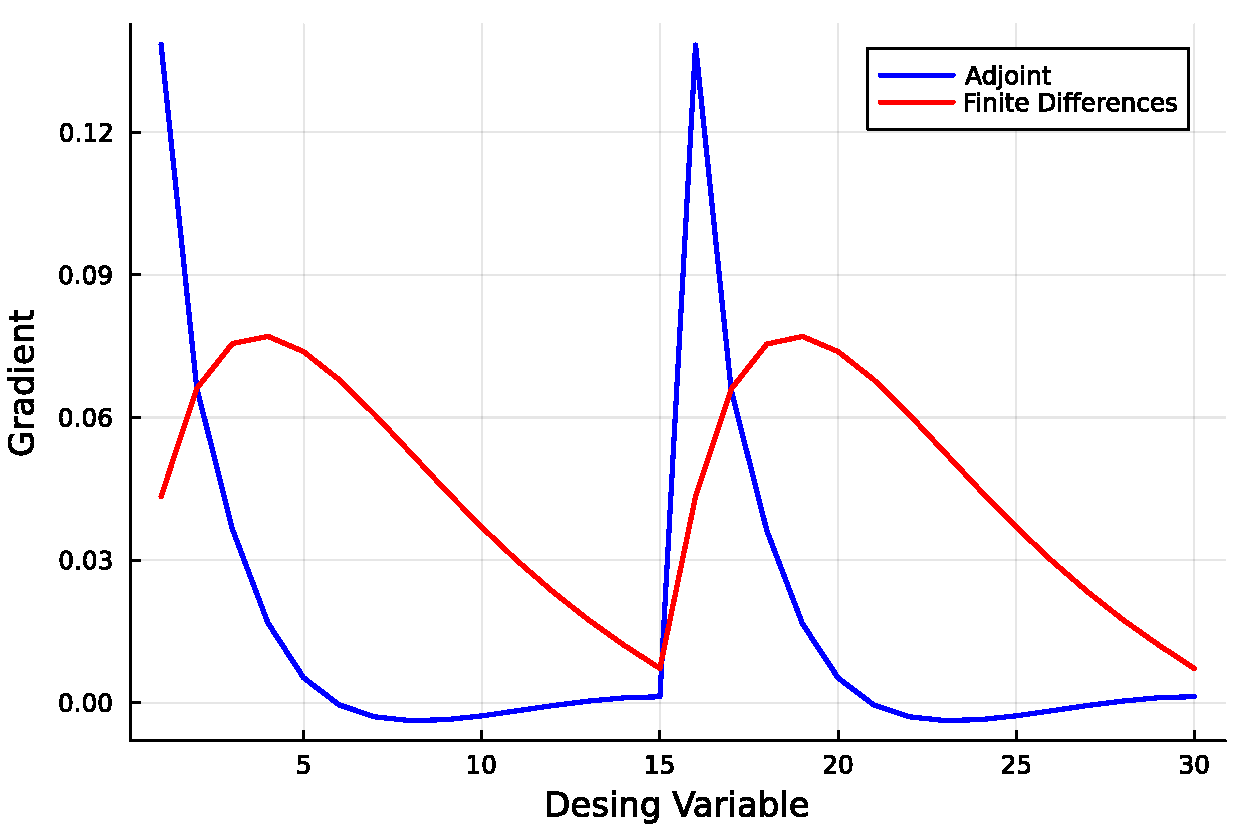
\includegraphics[width=0.3\textwidth]{Adjoint_FD.pdf}
       \caption{$C_D$ gradient, finite difference vs adjoint}
    \end{figure} 
\end{frame}

\begin{frame}{Finite Difference Tests}
Gradients are symmetric in top and bottom design variables
Order of magnitude really are close but not matching 
\end{frame}